\section{$\alpha$-Orientierungen}\label{alpha_orientations}

Für unseren Algorithmus in Kapitel \ref{main_algo} führen wir nun eine weitere zu Schnyder-Woods und Labelings in Bijektion stehende Struktur auf Graphen ein und halten uns dabei an \cite{felsner04}.

\begin{definition}[$\alpha$-Orientierung]
Sei $G=(V,E)$ ein ungerichteter Graph und $\alpha:V\mapsto\mathbb{N}$ eine Funktion auf $G$. Eine $\alpha$\textit{-Orientierung} ist eine Orientierung der Kanten von $G$, sodass der Ausgrad eines jeden Knoten $\alpha(v)$ entspricht. Somit muss gelten $$\text{outdeg}(v) = \alpha(v).$$
\end{definition}

Um von $\alpha$-Orientierungen zu Schnyder Woods zu gelangen müssen wir Primal-Dual Graphen betrachten die mit den nächsten beiden Definitionen eingeführt werden.

\begin{definition}[schwacher dualer Graph]
Sei $G$ ein planer Graph. $G^*$ der \textit{schwache duale Graph} von $G$. $G^*$ hat einen (Gebiets-)Knoten für jedes innere Gebiet von $G$. Für jede innerer Kante in $G$ fügen wir eine Kante zwischen den beiden (Gebiets-)Knoten $f,f'$ in $G^*$ ein, die adjazent zu dieser Kante in $G$ sind.
\end{definition}

\begin{definition}[Primal-Dual Graph]
Betrachte einen planen Graphen $G$ und seinen schwacher dualer Graphen $G^*$. Der \textit{Primal-Dual Graph} $G+G^*$ ist eine Vereinigung der Graphen $G$ und $G^*$ mit einem Knoten an jeder Kantenkreuzung. Die Menge der Knoten von $G+G^*$ besteht aus Knoten-Knoten, Kanten-Knoten und Gebiets-Knoten. Kanten in $G+G^*$ existieren, sowohl zwischen inzidenten Kanten und Knoten, als auch Kanten und Gebieten in $G$. Hinzu kommen Halbkanten\footnote{Kanten mit nur einem Randknoten die immer von diesem weg orientiert sind.} von den Kanten-Knoten und Knoten-Knoten am äusseren Gebiet von $G$.

Wenn wir einen Knoten $f_\infty$ für das äussere Gebiet hinzufügen und die Halbkanten zu diesem verlängern spricht man vom \textit{Abschluss} von $G+G^*$.

\end{definition}
Es ist leicht zu sehen, dass $G+G^*$ und sein Abschluss bipartit sind. Das folgende Theorem liefert eine Bijektion zwischen den Schnyder Woods auf $G$ und einer bestimmten $\alpha$-Orientierung auf $\tilde{G}$, die wir $\alpha_s$ nennen.

\begin{theorem}\label{alpha_bij}
Sei $G$ ein planer Graph mit Aufhängungen $\{a_1,a_2,a_3\}$, dann sind die folgenden Strukturen in Bijektion:
\begin{itemize}
\item [A1] Die Schnyder Woods auf $G$.
\item [A2] Die Schnyder Woods auf dem (schwachen) dualen Graphen $G^*$.
\item [A3] Die $\alpha_{s}$-Orientierungen des Abschlusses von $G+G^*$ mit $\alpha_s(v) = \alpha_s(f) = 3$ für jeden Knoten-Knoten $v$ und Gebiets-Knoten $f$,  $\alpha_s(e) = 1$ für jeden Kanten-Knoten $e$ und  $\alpha_s(f_\infty) = 0$.
\end{itemize}
\end{theorem}

\begin{remark}
Wir erhalten aus einem $\alpha_s$-Orientierung den Schnyder Wood, indem wir den drei Aufhängungen die Label rot, grün und blau geben und dann Schritt für Schritt die Kanten einfärben und dabei die Orientierung der Kanten aus $\alpha_s$ auf $G$ übernehmen erfüllen wir bereits W1 und W2. Wir nun an jedem Knoten an dem wir ankommen W3 bei der Einfärbung berücksichtigen erhalten wir einen eindeutigen Schnyder Wood auf $G$.
\end{remark}

\begin{figure}
	\centering
	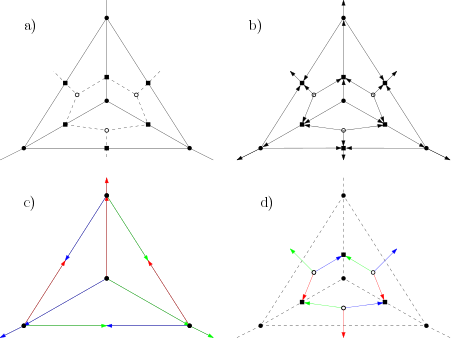
\includegraphics[width=1\textwidth]{alpha_ex2.png}
  \caption{Der Primal-Duale Graph $K_4+K_4^*$ mit einer $\alpha_s$-Orientiertung und den zugehörigen Schnyder Woods auf $K_4$ und $K^*_4$. }
\end{figure}